\documentclass[11pt]{article}

\usepackage[margin=1in]{geometry}
\usepackage[T1]{fontenc}
\usepackage{lmodern}
\usepackage{amsmath,amssymb}
\usepackage{graphicx}
\usepackage{booktabs}
\usepackage{tabularx}
\usepackage{threeparttable}
\usepackage{caption}
\usepackage{subcaption}
\usepackage[authoryear,round]{natbib}
\usepackage{xcolor}
\usepackage[colorlinks=true,linkcolor=blue!50!black,citecolor=blue!50!black,urlcolor=blue!50!black]{hyperref}
\usepackage{xurl}
\usepackage{float}
\usepackage{setspace}

\captionsetup{font=small,labelfont=bf}
\setstretch{1.08}

\newcommand{\E}{\mathbb{E}}
\newcommand{\CVaR}{\operatorname{CVaR}}

\title{Is an Electric Vehicle Insurance Against Gasoline Price Shocks?\\
\large A Two-Stage Stochastic Program for Chicago Rideshare Drivers}

\author{Veronica Guo\\
\small M.S. in Analytics, University of Southern California\\
\small ISE 599, Fall 2026}

\date{November 2026}

\begin{document}

\maketitle

\begin{abstract}
\noindent
Rideshare drivers pay for their own fuel, so a gasoline price shock lands directly on their income. A hybrid or a battery-electric vehicle (BEV) can be viewed as insurance: it costs more up front and should pay off when gasoline spikes. We test this view for a single Chicago rideshare driver who must choose between keeping an older gasoline car, buying a used hybrid, or buying a used BEV. We build the problem from public data: 94 months of trip records and monthly vehicle records from the City of Chicago, weekly Chicago gasoline prices since 2000, and Illinois electricity prices. Gasoline is modeled two ways, as a mean-reverting process with jumps and as a calm/crisis regime-switching process, and both are tested out of sample on the 2026 Iran-war shock. Electricity and revenue per hour are simulated jointly with gasoline. The car choice is the first stage of a two-stage stochastic program whose second stage allocates driving hours across 24 hourly blocks each month, subject to a time budget that includes charging and a cash constraint for the car payment. The objective trades off expected loss against the superquantile (CVaR) of the four-year loss. We find that a used hybrid dominates for drivers above roughly 60--75 hours a month, but mostly through steady fuel savings rather than tail protection. The largest risk to driver income is demand, not fuel, and a new car's fixed payment increases exposure to it, so risk aversion can favor keeping the old car. Without home charging, a fast-charged BEV never beats the hybrid for any average gasoline price between \$2 and \$9; with home charging it is the best choice for heavy and full-time drivers.
\end{abstract}

\noindent\textbf{Keywords:} stochastic programming; superquantile; conditional value-at-risk; regime switching; electric vehicles; ride-hailing; energy price shocks

\section{Introduction}

Gasoline prices in the United States have had two large shocks in five years. After Russia's invasion of Ukraine in 2022, the monthly average price of regular gasoline in Chicago rose above \$5.50 per gallon in June and fell back over the second half of the year. After the Iran war began at the end of February 2026, the Chicago monthly average went from \$2.97 in February to \$4.89 in May and was still \$4.73 in October \citep{eia2026,aljazeera2026,uchicago2026}. The first shock was a spike that reverted; the second has persisted.

Rideshare drivers are among the most exposed workers. Most own the car they drive \citep{seattle2016}, they pay for fuel, and platform fuel surcharges cover only part of a price jump \citep{uber2022}. A driver who switches to a hybrid or a battery-electric vehicle (BEV) pays more up front and lowers fuel cost per mile. If the main benefit appears in shock years, the newer car behaves like insurance, and the right question is how large the premium and the payout are, and for whom.

This paper studies that question for one driver at a time in Chicago. The driver owns an older gasoline car and chooses between keeping it, buying a used hybrid, or buying a used BEV. After the choice, prices and demand unfold over four years and the driver decides each month how many hours to drive and when. We formulate this as a two-stage stochastic program with a mean--superquantile objective \citep{rockafellar2000,rockafellar2002,royset2021} and build its inputs from public data.

The paper makes four contributions. First, we construct driver types, an hourly revenue curve and implied reservation wages from city trip and vehicle records, which gives the second stage a falling value of time rather than a linear one. Second, we compare two models of gasoline risk, a mean-reverting jump model and a regime model with labeled crisis periods, and evaluate both on the 2026 shock, which was held out of estimation. Third, we show that the tail of a driver's loss is driven by demand rather than fuel, so the hybrid's value is mainly in the mean and its fixed payment can make the tail worse; this creates a band of driving intensity in which the optimal car depends on risk aversion. Fourth, we show that home charging, not gasoline risk, determines whether a BEV is worth buying.

The rest of the paper is organized as follows. Section~\ref{sec:lit} reviews related work. Section~\ref{sec:data} describes the data, the powertrain classification and the driver types. Section~\ref{sec:uncertainty} presents the price and demand models and their out-of-sample test. Section~\ref{sec:model} states the optimization model. Section~\ref{sec:results} reports results, Section~\ref{sec:discussion} discusses limitations, and Section~\ref{sec:conclusion} concludes. Appendix~\ref{app:params} lists parameters and Appendix~\ref{app:ai} describes how AI tools were used and checked.

\section{Related Literature}\label{sec:lit}

\paragraph{Risk-averse stochastic programming.} Two-stage stochastic programs with recourse are standard for decisions made before uncertainty is resolved \citep{birge2011}. The superquantile, also called conditional value-at-risk, measures the average of the worst outcomes beyond a quantile and has a convex, linear-programming representation \citep{rockafellar2000,rockafellar2002}. \citet{royset2021} treat superquantile-based risk measures within a general optimization framework. Large scenario sets are often reduced before optimization; \citet{heitsch2003} give reduction methods based on probability metrics. We use a simpler clustering reduction and check that it preserves the tail.

\paragraph{Energy price dynamics.} Commodity prices tend to revert toward a long-run level \citep{schwartz1997}, and jump components capture sudden moves \citep{merton1976}. Regime-switching models, introduced by \citet{hamilton1989}, allow parameters to change between calm and turbulent periods. \citet{kilian2008} reviews how energy price shocks reach households. Our contribution here is applied: we compare a jump model and a regime model on the same data and judge them by a held-out shock.

\paragraph{Ride-hailing labor.} \citet{cramer2016} estimate that UberX drivers carry a passenger for about half of their logged-in time. \citet{hall2018} describe drivers' hours and earnings, and \citet{chen2019} show that drivers place substantial value on flexible scheduling, which supports our use of reservation wages below the local minimum wage.

\section{Data}\label{sec:data}

\subsection{Sources}

Table~\ref{tab:data} lists the data. The City of Chicago publishes monthly records for every vehicle used by a transportation network provider (TNP), with make, model, model year and number of trips, and trip-level records with fare, tip, distance, duration and start time \citep{chicagotnp}. We aggregated trips by month and hour of day for November 2018 through September 2026 (94 months). Gasoline prices are weekly Chicago retail regular prices from June 2000; electricity is the monthly Illinois average retail price \citep{eia2026}. Fuel economy and the list of powertrains sold under each model name come from \citet{epa2026}.

\begin{table}[ht]
\centering
\caption{Data sources.}\label{tab:data}
\small
\begin{tabularx}{\textwidth}{@{}l l X@{}}
\toprule
Dataset & Coverage & Use \\
\midrule
TNP Vehicles (Chicago) & 2015--2026, monthly & Fleet composition; trips per vehicle; driver types \\
TNP Trips (Chicago) & Nov 2018--Sep 2026 & Fare, tips, miles and time by month and hour of day \\
Taxi licenses (Chicago) & current & Recorded fuel type; test set for labels \\
Retail gasoline, Chicago (EIA) & Jun 2000--Oct 2026, weekly & Gasoline price models \\
Retail electricity, Illinois (EIA) & 2001--Aug 2026, monthly & Charging cost; link to gasoline \\
Fuel economy (EPA) & model years 1984--2026 & MPG, kWh/mile, powertrains by model and year \\
\bottomrule
\end{tabularx}
\end{table}

\subsection{Powertrain classification}

The vehicle records have no trim field, so a model name such as ``Camry'' may refer to a gasoline or a hybrid car. We assign each make, model and model year a label in three passes: (i) a name rule (for example ``Prius'', ``Hybrid'', ``Bolt''); (ii) the EPA table for that make, model and model year (within one year), which lists every powertrain sold under the name; and (iii) a large language model for strings that EPA cannot match. When EPA lists more than one powertrain, the row is labeled ambiguous and the hybrid share is reported as a range. Mild hybrids with systems below 160\,V are treated as gasoline vehicles because they cannot drive on electric power and have similar fuel economy.

We validate the labels on Chicago taxis, whose licenses record the actual fuel type. Rows with a single label are correct 97.0\% of the time, and for ambiguous rows the true fuel type is among the listed options 99.9\% of the time. A hand check of 296 sampled rows found three systematic errors (mild hybrids, plug-in models sold under a ``Hybrid'' name, and model-year mismatches in the language-model labels), which were corrected.

Figure~\ref{fig:fleet} shows the resulting fleet mix. BEVs rose from 0.2\% of active vehicles in September 2020 to 2.3\% in September 2022 and 4.9\% in September 2026. Hybrids made up between 24.7\% and 45.9\% in September 2026.

\begin{figure}[ht]
\centering
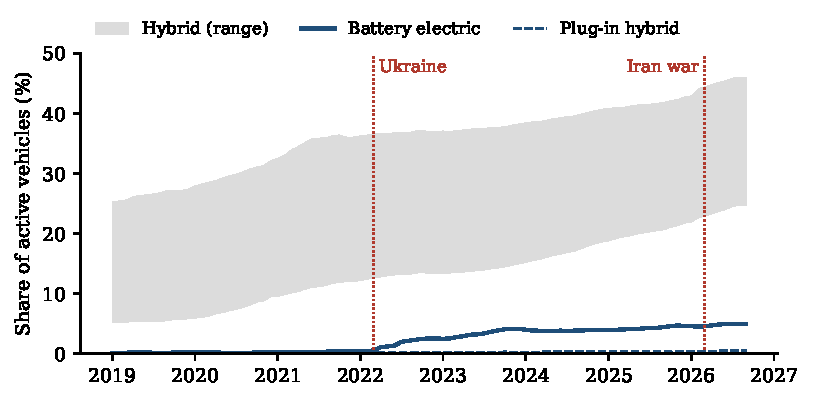
\includegraphics[width=0.85\textwidth]{figures/fleet_share.pdf}
\caption{Powertrain mix of active Chicago TNP vehicles. The hybrid band runs from vehicles labeled hybrid (lower edge) to those plus ambiguous models that were also sold as hybrids (upper edge).}\label{fig:fleet}
\end{figure}

\subsection{Driver types and the hourly revenue curve}

The data identify vehicles, not drivers, so we treat a vehicle-month as a driver-month. Using October 2025--September 2026, we group vehicles by trips per month (Table~\ref{tab:types}). About 21\% of vehicles provide 59\% of trips.

Logged-in hours are not observed. We convert trip time into logged-in time using a utilization rate of 0.5 on average \citep{cramer2016}, scaled up in busy hours with elasticity 0.3 to hourly demand. Miles include empty driving, using a paid-mile share of 0.58 \citep{fehrpeers2019}. The full-time group averages 361 logged-in hours per vehicle-month, more than one person can drive, so we cap a driver at 60 hours per week (260 per month) and treat the rest as vehicle sharing.

For each of the 24 clock hours $b$ we compute the driver's revenue per logged-in hour, $\mathit{rev}_b$, as the driver's share of fares (0.65) plus tips (9.3\% of fares in 2026), and miles per logged-in hour, $m_b$ (Figure~\ref{fig:rev}). Revenue ranges from about \$21 per hour between 9\,p.m.\ and midnight to about \$15 between 2 and 4\,a.m. A driver fills the best hours first, so the value of an additional hour falls.

\begin{figure}[ht]
\centering
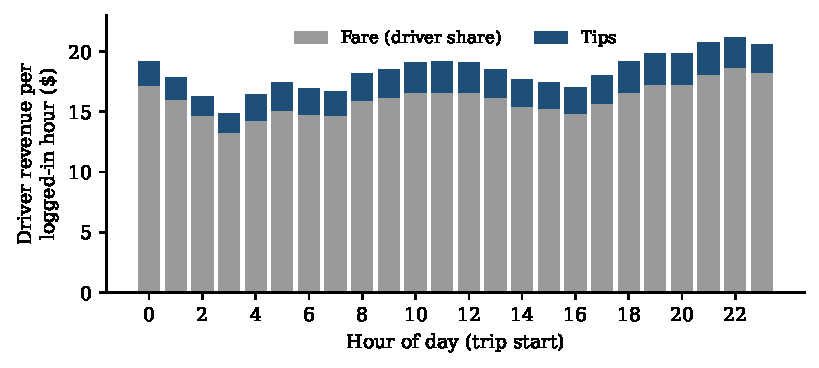
\includegraphics[width=0.85\textwidth]{figures/revenue_by_hour.pdf}
\caption{Driver revenue per logged-in hour by hour of day, October 2025--September 2026.}\label{fig:rev}
\end{figure}

\subsection{Reservation wages}

Net of fuel and maintenance for the current gasoline car, an hour of driving is worth \$10--\$16, below Chicago's \$17.05 minimum wage. Using the minimum wage as the outside option would imply that no one drives. Following the evidence that drivers value flexibility \citep{chen2019}, we instead infer a reservation wage $r$ for each type: assuming today's hours are optimal, $r$ equals the net value of the marginal hour at today's hours. Heavier drivers have lower reservation wages (Table~\ref{tab:types}). In the model a driver may increase hours by up to 20\%, subject to the 260-hour cap.

\begin{table}[ht]
\centering
\caption{Driver types, October 2025--September 2026.}\label{tab:types}
\small
\begin{tabular}{@{}lrrrrrr@{}}
\toprule
Type & Trips/month & Vehicles (\%) & Trips (\%) & Hours/month & Miles/month & $r$ (\$/h) \\
\midrule
Light & 1--50 & 42.3 & 6.4 & 12 & 265 & 15.42 \\
Regular & 51--200 & 36.9 & 34.8 & 76 & 1{,}651 & 14.99 \\
Heavy & 201--400 & 16.0 & 37.2 & 188 & 3{,}883 & 13.89 \\
Full-time & $>400$ & 4.8 & 21.6 & 260 & 5{,}265 & 13.77 \\
\bottomrule
\end{tabular}
\end{table}

\section{Modeling Uncertainty}\label{sec:uncertainty}

All models are estimated on data through December 2025. Data from 2026 are used only for evaluation.

\subsection{Gasoline: preliminaries}

Let $p_t$ be the gasoline price and $x_t = \log p_t - s_{w(t)}$ the log price net of a seasonal factor for week (or month) of year, estimated as the average deviation from a centered one-year moving average. Chicago prices are about 20\% higher in early summer than in December. Both models revert toward a log-linear trend. The estimation window matters: starting in 2000 yields a trend of 2.8\% per year, driven by low prices in the early 2000s, and an end-2025 trend level of \$3.87, well above observed prices; both models then drift upward in 2026 for reasons unrelated to shocks. We therefore estimate from January 2005, which gives a trend of about 1.0\% per year and an end-2025 level near \$3.30.

\subsection{Model A: mean reversion with jumps}

On weekly data,
\begin{equation}\label{eq:jump}
\Delta x_t = c + g\,t - \kappa\, x_{t-1} + \phi\, \Delta x_{t-1} + \sigma \varepsilon_t + J_t,
\end{equation}
where $\varepsilon_t$ is standard normal and $J_t$ is an upward jump $N(\mu_u,\sigma_u^2)$ with probability $\pi_u$, a downward jump $N(\mu_d,\sigma_d^2)$ with probability $\pi_d$, and zero otherwise \citep{merton1976,schwartz1997}. We estimate by a robust filter: fit~\eqref{eq:jump} without jumps by least squares, flag residuals beyond three robust standard deviations (median absolute deviation) as jumps, refit on the remaining weeks, and repeat until the flagged set is stable. The half-life of a deviation is 55 weeks, the momentum coefficient is $\phi = 0.23$, upward jumps occur 0.43 times per year with mean size $+12.0\%$, and downward jumps 0.24 times per year with mean $-9.2\%$.

\subsection{Model B: calm and crisis regimes}

We first estimated a two-regime Markov switching model by maximum likelihood \citep{hamilton1989}. The high-volatility regime it identified consisted of price collapses (late 2008, 2015, spring 2020) rather than periods of persistently high prices. To capture the latter, we label crisis months from supply shocks that were known before 2026: Hurricanes Katrina and Rita (September--November 2005), the 2008 oil price spike (March--August 2008), the Libyan civil war (February--July 2011), Iran sanctions and Strait of Hormuz threats (February--May 2012), and the Russian invasion of Ukraine (March--August 2022). On monthly data, with $z_t$ the deviation of $x_t$ from trend and regime $k_t \in \{\text{calm}, \text{crisis}\}$,
\begin{equation}\label{eq:regime}
\Delta x_t = a_{k_t} + b_{k_t}\, z_{t-1} + \phi_{k_t}\, \Delta x_{t-1} + \sigma_{k_t} \varepsilon_t ,
\end{equation}
estimated by least squares within each regime. Regimes follow a Markov chain whose entry and exit rates match the frequency and length of the labeled crises. A crisis begins 0.27 times per year, lasts 5.0 months on average, and pulls prices toward a level $-a/b \approx 26\%$ above trend.

\subsection{Out-of-sample test on 2026}

We simulated 5{,}000 paths of each model from the last week of 2025 (Figure~\ref{fig:backtest}, Table~\ref{tab:backtest}). Neither model rules out 2026, but both treat it as roughly a one-in-ten-year event. The May peak of \$4.89 falls at the 98th (A) and 96th (B) percentile, and the October price of \$4.73 at the 96th percentile under both. The persistence of high prices after the spring peak is the feature both models understate.

\begin{figure}[ht]
\centering
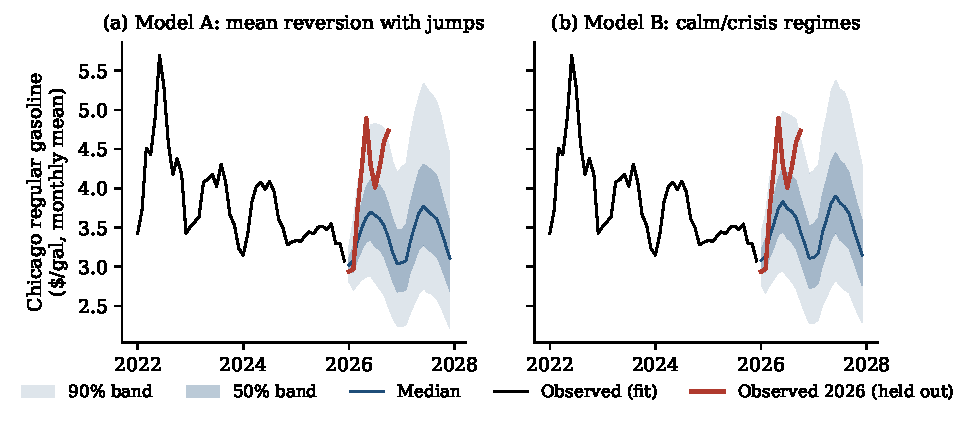
\includegraphics[width=\textwidth]{figures/gas_backtest.pdf}
\caption{Simulated gasoline price distributions from January 2026 (fit on 2005--2025) against observed prices. The red line was not used in estimation.}\label{fig:backtest}
\end{figure}

\begin{table}[ht]
\centering
\caption{Out-of-sample evaluation on 2026.}\label{tab:backtest}
\small
\begin{tabular}{@{}lcc@{}}
\toprule
 & Model A & Model B \\
\midrule
$P$(some 2026 month averages $\geq$ \$4.50) & 0.19 & 0.25 \\
$P$(Mar--Oct 2026 mean $\geq$ observed \$4.35) & 0.08 & 0.10 \\
Percentile of observed May 2026 (\$4.89) & 98 & 96 \\
Percentile of observed October 2026 (\$4.73) & 96 & 96 \\
\bottomrule
\end{tabular}
\end{table}

\subsection{Electricity and revenue}

\paragraph{Electricity.} The DC fast-charging price is scaled by the Illinois commercial electricity price. Regressing 12-month log changes of electricity on those of gasoline over 2015--2025 gives an elasticity of 0.12 ($t = 2.0$, Newey--West standard errors; \citealp{newey1987}). Electricity also drifted up 3.7\% per year. We simulate the log electricity index as drift plus the gasoline link plus an AR(1) component and a random walk with 5\% annual standard deviation.

\paragraph{Revenue.} Let $R_t$ be an index of revenue per logged-in hour (fare per trip-hour times utilization). Over 2022--2025 its elasticity to gasoline is 0.20 ($t = 2.2$), but this reflects the post-pandemic recovery of demand coinciding with high 2022 prices; in 2026 revenue per hour fell about 10\% year over year while gasoline rose. The base case therefore sets the link to zero and gives $R_t$ a seasonal factor, an AR(1) component and a random walk with about 4\% annual standard deviation. Links of $-0.3$ and $+0.2$ are sensitivity cases.

\subsection{Scenario generation and reduction}

For each gasoline model we simulate 5{,}000 joint 48-month paths of gasoline, electricity and revenue and reduce them to $|S| = 300$ scenarios by $k$-means clustering on standardized log paths, keeping the path nearest each centroid and assigning it the cluster's probability. The reduction preserves the tail: under Model A the 90th percentile of the four-year mean gasoline price is \$4.12 in the reduced set and \$4.14 in the full set.

\section{Optimization Model}\label{sec:model}

\subsection{Decisions and parameters}

The first-stage decision is $x \in X = \{\text{keep}, \text{hybrid}, \text{BEV}\}$: keep a 2018 Toyota Camry LE (trade-in value \$13{,}000), buy a 2023 Camry Hybrid LE (\$26{,}000), or buy a 2023 Tesla Model~3 RWD (\$25{,}000). A purchase is financed over 48 months at 8.8\% APR with the trade-in as down payment. Appendix~\ref{app:params} lists all parameters.

In the second stage, for scenario $s \in S$ with probability $p_s$, month $t = 1,\dots,48$ and clock-hour block $b = 1,\dots,24$, the driver chooses hours $h_{stb} \geq 0$ and short-term borrowing $w_{st} \geq 0$. Let $c_{x,st}$ be the cost per mile of car $x$ (fuel or charging plus maintenance), $\tau_x$ the charging hours per mile (positive only for a BEV without home charging: 30 minutes per 175 miles, rising with battery fade), $r$ the reservation wage, $\kappa = 0.15$ the cost per dollar borrowed, $P_x$ the monthly loan payment plus insurance, $F_x = 48P_x$ and $V_x$ the resale value after four years.

\subsection{Formulation}

The loss in scenario $s$ is the negative of the driver's four-year surplus:
\begin{equation}\label{eq:loss}
L_x(s) = \sum_{t=1}^{48}\Big[-\sum_{b=1}^{24} h_{stb}\big(\mathit{rev}_b R_{st} - m_b\, c_{x,st} - r\,(1+\tau_x m_b)\big) + \kappa\, w_{st}\Big] + F_x - V_x .
\end{equation}
For each $s$ and $t$,
\begin{align}
\sum_{b} h_{stb}\,(1+\tau_x m_b) &\leq H_{\max}, \label{eq:time}\\
0 \leq h_{stb} &\leq 30.4, \label{eq:avail}\\
\sum_{b} h_{stb}\big(\mathit{rev}_b R_{st} - m_b\, c_{x,st}\big) - P_x + w_{st} &\geq N, \label{eq:cash}
\end{align}
where~\eqref{eq:time} is the time budget, in which charging time consumes driving time;~\eqref{eq:avail} limits each clock hour to the number of times it occurs in a month; and~\eqref{eq:cash} requires driving income net of car costs to cover the amount $N$ the driver relies on (85\% of current net driving income), with any shortfall borrowed.

The driver solves
\begin{equation}\label{eq:obj}
\min_{x \in X}\; (1-\lambda)\, \E\big[L_x\big] + \lambda\, \CVaR_\alpha\big(L_x\big), \qquad \alpha = 0.9,\; \lambda \in [0,1],
\end{equation}
with the superquantile computed by the Rockafellar--Uryasev formula \citep{rockafellar2000}:
\begin{equation}\label{eq:ru}
\CVaR_\alpha(L_x) = \min_{\eta \in \mathbb{R}}\; \eta + \frac{1}{1-\alpha}\sum_{s \in S} p_s\, \big[L_x(s) - \eta\big]_+ ,
\end{equation}
linearized with auxiliary variables $u_s \geq L_x(s) - \eta$, $u_s \geq 0$.

\subsection{Why the second stage is not trivial}

With constant revenue and cost per hour, the recourse would be all-or-nothing. Three features prevent this. First, the hourly revenue curve makes the value of time decreasing, so a gasoline-car driver can absorb a price shock by dropping the least valuable hours. Second, a purchased car carries a fixed payment $P_x$, whereas the old car has almost none; the old car therefore retains the option to drive less in a bad month without a cash shortfall. Third, without home charging a BEV loses driving time to charging in~\eqref{eq:time}, which matters most for the drivers who would save the most on fuel.

\subsection{Solution method and verification}

Because $|X| = 3$, we solve the second-stage linear program for each car (300 scenarios $\times$ 48 months $\times$ 24 blocks, about 360{,}000 variables) with HiGHS \citep{huangfu2018} and compare objectives; this is equivalent to the mixed-integer program with binary first-stage variables. Since lowering the loss in any scenario weakly lowers both the expectation and the superquantile, the recourse that minimizes each scenario's loss is optimal for every $\lambda$, so a single solve per car serves all $\lambda$. We verified the implementation in three ways: the LP matches a hand-computed greedy solution in a one-month case; at $\lambda = 1$ the LP objective equals the superquantile computed directly from its scenario losses; and the full Rockafellar--Uryasev LP at $\lambda = 0.5$ reproduces the objective of the one-solve approach.

\section{Results}\label{sec:results}

\subsection{Base case}

Table~\ref{tab:base} reports the base case: used cars, no home charging, no subsidies, Model A scenarios. Light drivers should keep the gasoline car; regular, heavy and full-time drivers should buy the hybrid. The BEV is never optimal. The choice does not change between $\lambda = 0$ and $\lambda = 1$ for any type, and Model B changes the values by less than \$600.

\begin{table}[ht]
\centering
\caption{Base case: four-year gain in driver surplus (thousands of dollars). Positive values favor the second car.}\label{tab:base}
\small
\begin{threeparttable}
\begin{tabular}{@{}llrrr@{}}
\toprule
Type & Optimal car & Hybrid vs.\ keep, $\E$ & Hybrid vs.\ keep, $\CVaR_{0.9}$ & BEV vs.\ hybrid, $\E$ \\
\midrule
Light & Keep & $-7.0$ & $-7.4$ & $-6.2$ \\
Regular & Hybrid & $1.6$ & $0.3$ & $-14.0$ \\
Heavy & Hybrid & $13.2$ & $11.7$ & $-25.9$ \\
Full-time & Hybrid & $16.9$ & $16.2$ & $-29.7$ \\
\bottomrule
\end{tabular}
\begin{tablenotes}\footnotesize
\item Surplus is net driving income minus time valued at the reservation wage, minus car costs, plus resale value. The $\CVaR$ column compares the average of the worst 10\% of scenarios for each car.
\end{tablenotes}
\end{threeparttable}
\end{table}

\subsection{When risk aversion changes the choice}

Figure~\ref{fig:sweep} varies baseline driving time from 10 to 260 hours per month, with reservation wages inferred at each level. The hybrid's expected gain turns positive at about 62 hours per month, but its gain in the worst 10\% of scenarios turns positive only at about 73 hours. Between the two, a risk-neutral driver buys the hybrid and a sufficiently risk-averse driver keeps the old car.

This runs against the insurance interpretation. The worst 10\% of scenarios are not those with the highest gasoline prices: revenue per hour is about 7.5\% below normal in them, while gasoline is only slightly above average. For a heavy driver the standard deviation of four-year revenue is roughly three times that of four-year fuel cost. The hybrid lowers fuel risk, but its fixed payment binds hardest in low-demand months, which raises exposure to the larger risk. The old car's option to drive less is worth more in the tail than the hybrid's fuel hedge.

\begin{figure}[ht]
\centering
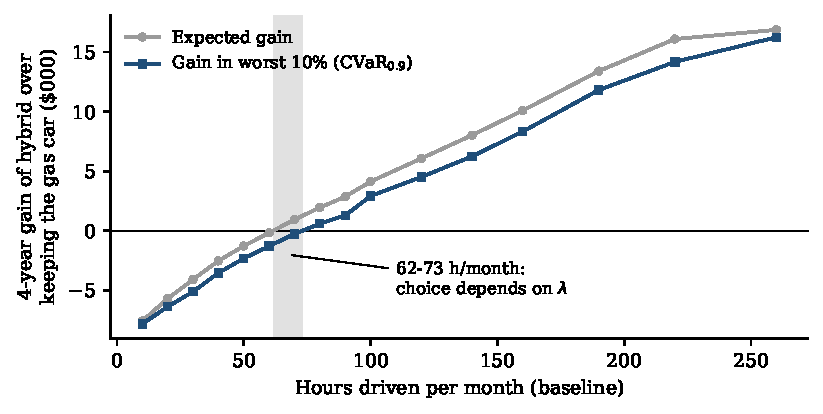
\includegraphics[width=0.85\textwidth]{figures/hybrid_sweep.pdf}
\caption{Four-year gain of the hybrid over keeping the gasoline car, by baseline hours per month (Model A). Gray band: range where the optimal car depends on $\lambda$.}\label{fig:sweep}
\end{figure}

The BEV loses because, on DC fast chargers at \$0.50/kWh, its cost per mile including maintenance (about \$0.21) exceeds the hybrid's (about \$0.16 at \$3.55 gasoline), a heavy driver spends about 11 hours per month charging, and the BEV has lower resale value and higher insurance. The gap widens with mileage.

\subsection{Sensitivity}

Table~\ref{tab:sens} reports the optimal car under alternative assumptions. Home charging is the assumption that matters for the BEV: with it, the BEV beats the hybrid by about \$5{,}700 over four years for heavy drivers and \$7{,}200 for full-time drivers. Purchase subsidies alone (\$2{,}000 Illinois rebate plus \$4{,}000 Uber grant) or cheaper fast charging do not change the base result. Risk aversion changes the regular driver's choice when the fixed payment becomes more costly (a 13.9\% APR) or when revenue falls with gasoline, as it did in 2026.

\begin{table}[ht]
\centering
\caption{Optimal car under alternative assumptions. ``A/B'' gives the choice at $\lambda=0$ / $\lambda=1$ when they differ.}\label{tab:sens}
\small
\begin{tabular}{@{}lllll@{}}
\toprule
Case & Light & Regular & Heavy & Full-time \\
\midrule
Base (Model A) & Keep & Hybrid & Hybrid & Hybrid \\
Gasoline Model B & Keep & Hybrid & Hybrid & Hybrid \\
Home charging & Keep & Hybrid/BEV & BEV & BEV \\
Home charging + \$6k subsidies & Keep & BEV & BEV & BEV \\
New BEV (\$37k) + home charging + subsidies & Keep & Hybrid & BEV & BEV \\
Subsidies only & Keep & Hybrid & Hybrid & Hybrid \\
DC fast charging at \$0.40/kWh & Keep & Hybrid & Hybrid & Hybrid \\
Loan APR 13.9\% & Keep & Hybrid/Keep & Hybrid & Hybrid \\
Revenue elasticity to gasoline $-0.3$ & Keep & Hybrid/Keep & Hybrid & Hybrid \\
Revenue elasticity to gasoline $+0.2$ & Keep & Hybrid & Hybrid & Hybrid \\
\bottomrule
\end{tabular}
\end{table}

\paragraph{Break-even gasoline prices.} Scaling every gasoline path, a regular driver prefers the hybrid once the four-year mean price exceeds about \$2.16, compared with a forecast mean of \$3.53. A light driver keeps the old car for any mean between \$2 and \$9. Without home charging the BEV never beats the hybrid in that range: relative to a hybrid, a fast-charged BEV is not insurance at any plausible gasoline price.

\subsection{Ex-post evaluation on 2026}

We ran each car through the observed January--September 2026 path, with car costs spread evenly over the four-year horizon. Gasoline rose from \$2.94 to \$4.59, revenue per hour fell about 6\%, and commercial electricity rose 18\%. Every car's outcome fell between the 3rd and 10th percentile of the model's forecast for those months. The hybrid beat the gasoline car by about \$2{,}100 for heavy drivers and \$2{,}600 for full-time drivers, slightly less than expected (\$2{,}500 and \$3{,}000). The shock did not raise the hybrid's advantage, because lower revenue led drivers to cut hours and therefore fuel use. The BEV underperformed its forecast because electricity prices also rose.

\subsection{Implied versus actual fleet}

Weighting types by their share of vehicles, the base case implies a fleet of 42\% gasoline and 58\% hybrid vehicles; with universal home charging, 42\% gasoline, 37\% hybrid and 21\% BEV. The observed fleet in September 2026 was about 70\% gasoline (including ambiguous models), 24.7--45.9\% hybrid and 4.9\% BEV. The observed hybrid share lies between the two model cases and the low BEV share is consistent with limited home charging. The model implies far fewer gasoline cars than observed. Likely reasons are staggered replacement cycles, credit constraints at the assumed interest rate, and drivers not evaluating the decision in these terms.

\section{Discussion and Limitations}\label{sec:discussion}

The main uncertainty in our conclusions lies in the revenue model and in car costs rather than in the gasoline model. The revenue random walk is estimated from four post-pandemic years, and the sign of its relation to gasoline changed between 2022 and 2026. If revenue risk is larger than assumed, the case for keeping the old car strengthens; if smaller, the hybrid looks better still.

Purchase prices, maintenance, insurance and resale values come from outside sources. Resale value is the most uncertain, since a full-time driver accumulates close to 250{,}000 miles in four years.

Only five crises are labeled in 21 years, so crisis frequency and size are imprecise, and the 2026 test suggests that historically fitted models understate how long a shock can last.

We model driver types rather than individuals. A vehicle-month proxies for a driver-month, and the data contain no persistent vehicle identifier, outside income, home-charging access or credit information. Reservation wages are inferred from the assumption that current hours are optimal. The hybrid share is a range because trims are not recorded. Finally, we do not discount and ignore taxes; discounting would slightly favor keeping the old car, since purchase costs come early and resale value comes at the end.

\section{Conclusion}\label{sec:conclusion}

For a Chicago rideshare driver without home charging, a battery-electric vehicle is not insurance against gasoline price shocks: a used hybrid costs less per mile than a fast-charged BEV at any plausible gasoline price. The hybrid is the better car for drivers above roughly 60--75 hours per month, but its value comes from steady fuel savings rather than from payouts in a crisis, and its fixed payment raises exposure to the larger risk, which is demand. This produces a range of driving intensity where the optimal car depends on risk attitude. With home charging, the BEV becomes the best choice for heavy and full-time drivers, and with subsidies for regular drivers as well. For policy, this suggests that charging access where drivers live would do more to electrify rideshare fleets than larger purchase rebates. For drivers, the 2026 experience shows that gasoline, demand and electricity can move together, and the car that held up best was the one that lowered running costs without adding much fixed cost.

\section*{Data and Code Availability}

All data are public. Code for data retrieval, labeling, estimation, scenario generation and optimization, along with the intermediate results reported here, is available in the project repository.

\clearpage
\bibliographystyle{plainnat}
\bibliography{references}

\clearpage
\appendix

\section{Parameters}\label{app:params}

\begin{table}[H]
\centering
\caption{Vehicle parameters (base case).}\label{tab:params}
\small
\begin{threeparttable}
\begin{tabular}{@{}lrrr@{}}
\toprule
Parameter & Keep & Hybrid & BEV \\
\midrule
Representative model & 2018 Camry LE & 2023 Camry Hybrid LE & 2023 Model 3 RWD \\
Purchase price (\$) & -- & 26{,}000 & 25{,}000\tnote{a} \\
Trade-in value now (\$) & 13{,}000 & 13{,}000 & 13{,}000 \\
Fuel economy (EPA combined) & 34 mpg & 52 mpg & 0.255 kWh/mi \\
City factor / charging loss & $\times 0.85$ & $\times 1.00$ & $+10\%$ \\
Maintenance (\$/mi) & 0.13 & 0.09 & 0.06 \\
Resale after 4 years & \$3{,}000 & 45\% of price & 30\% of price \\
Insurance (\$/yr)\tnote{e} & 1{,}944 & 1{,}944 & 2{,}283 \\
Loan & -- & 48 mo., 8.8\%\tnote{b} & 48 mo., 8.8\%\tnote{b} \\
Fast charging & -- & -- & 30 min/175 mi\tnote{c} \\
Charging price (\$/kWh) & -- & -- & 0.50\tnote{d} \\
\bottomrule
\end{tabular}
\begin{tablenotes}\footnotesize
\item[a] \$37{,}000 in the new-BEV case. \item[b] 13.9\% APR in the high-rate case. \item[c] Range added falls with battery fade of 3\% per year. \item[d] DC fast charging, scaled by the electricity index; \$0.17 in the home-charging case. \item[e] Includes a \$250 rideshare endorsement; BEV premium assumed 20\% higher.
\end{tablenotes}
\end{threeparttable}
\end{table}

\begin{table}[H]
\centering
\caption{Market and model parameters (base case).}\label{tab:params2}
\small
\begin{tabular}{@{}lrl@{}}
\toprule
Parameter & Value & Source or range \\
\midrule
Driver share of fare & 0.65 & 0.50--0.79 \\
Paid-mile share & 0.58 & \citet{fehrpeers2019} \\
Mean utilization of logged-in time & 0.50 & \citet{cramer2016} \\
Utilization elasticity to hourly demand & 0.3 & 0--0.6 \\
Maximum hours per driver & 260/month & 60 per week \\
Hours flexibility above baseline & 20\% & \\
Borrowing cost $\kappa$ & 0.15 per \$ & \\
Cash need $N$ & 85\% & of current net driving income \\
Superquantile level $\alpha$ & 0.90 & \\
Horizon & 48 months & \\
Scenarios & 300 & reduced from 5{,}000 \\
\bottomrule
\end{tabular}
\end{table}

\section{Use of AI Tools}\label{app:ai}

An AI assistant was used throughout: to frame the model, write the data pipeline and optimization code, label vehicle powertrains and locate sources. Each use was checked against data or independent calculations, and Table~\ref{tab:ai} records the errors found.

\begin{table}[H]
\centering
\caption{AI use, checks and errors found.}\label{tab:ai}
\small
\begin{tabularx}{\textwidth}{@{}l X X@{}}
\toprule
Task & Check & Errors found and fixes \\
\midrule
Model formulation & Instructor review & First second stage (choose total hours) was trivial under linear revenue and cost; added a decreasing hourly revenue curve, fixed versus variable cost, charging time and a cash constraint \\
Powertrain labels & Taxi fuel types; 296-row hand audit & Language model ignored model year; EPA labels 48\,V mild hybrids as hybrids; plug-ins sold under a ``Hybrid'' name \\
Parameter research & Opened every cited source & A 2022 rental program was misread as a driver purchase subsidy \\
Gasoline models & Held-out 2026 test & 2000 start date built in a spurious trend; maximum-likelihood regimes captured crashes rather than crises \\
Calibration & Comparison with observed hours & Minimum wage as outside option implied zero driving; replaced by inferred reservation wages \\
Code & Hand-computed cases and identities & A constant was omitted from the reported objective; caught by comparing the full Rockafellar--Uryasev LP with the one-solve approach \\
\bottomrule
\end{tabularx}
\end{table}

\end{document}
